\documentclass{article}
\usepackage{amsmath}
\usepackage{amssymb}
\usepackage[hmargin=1.8cm,vmargin=2.5cm]{geometry}
\usepackage{tabularx}
\usepackage{booktabs}
\usepackage{graphicx}
\usepackage{color}
\usepackage{wrapfig}
\usepackage{multirow}
\usepackage{multicol}
\usepackage{cite}
\usepackage[rightcaption]{sidecap}
%\usepackage{hyperref}
\usepackage{threeparttable}
\usepackage[table]{xcolor}
\usepackage{psfrag}
\usepackage[margin=10pt,font=small,textfont=sf,labelfont=bf]{caption}
\usepackage{subfig}
\usepackage[section]{placeins}

\title{CDMS SNOLab Tower Hardware}
\author{Nicholas Kellaris and Miguel Daal}
\begin{document}
\bibliographystyle{plain}
\maketitle

\section{Phonon Readout Cable}

\subsection{Thermal Conductivity of Kapton Polyimide}

Thermal conductivity data for Kapton varies among the literature, as can be seen from Figure 1. In particular, we are interested in the Kapton HN data, as the company fabricating our stripline, Tech-Etch, uses this type. The power law fit of these thermal conductivities in the range of interest is presented in Table 1. The thermal conductivity used in heat load calculations was the data from M. Barucci \cite{bar}. This thermal conductivity is markedly higher than most of the other data. this is likely due to the direction of measurement along the sample. Barucci measures along a strip of Kapton, while other authors use a laminate of Kapton strips and measure through the thickness of the laminate (transverse to the Kapton strip direction). Unless the Kapton is isotropic, this would result in a different measured thermal conductivity.

\begin{figure}[h]
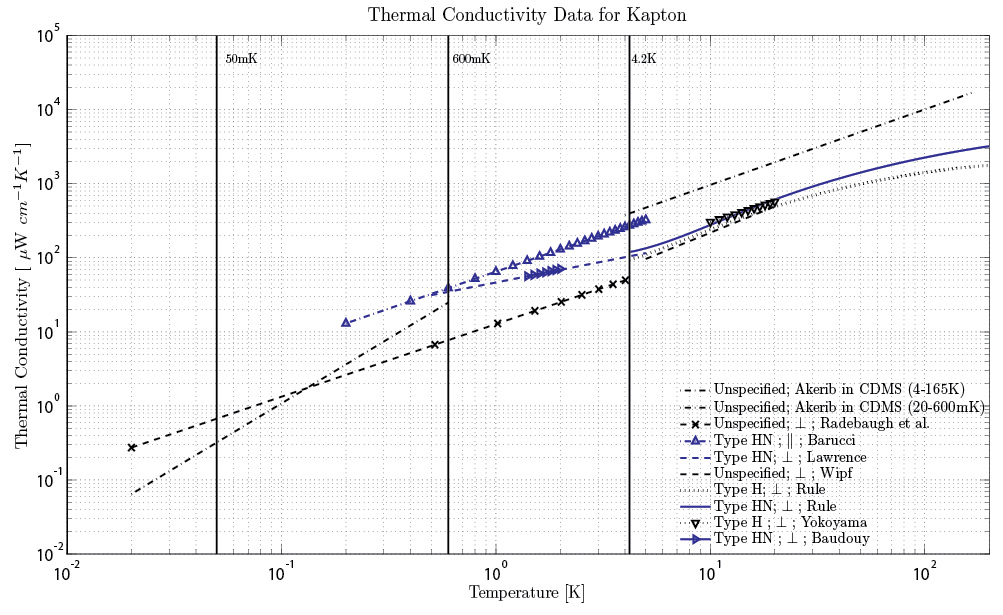
\includegraphics[width = .9\textwidth]{Kapton_var.png}
\caption{Compiled data for the thermal conductivity of Kapton films. The type is specified in the legend, as well as whether measurements were performed parallel or perpendicular to the Kapton surface. The direction of Kapton measurement is not stated when unknown. Data are from Radebaugh \cite{rad73}, Barucci \cite{bar}, Lawrence \cite{law}, Wipf \cite{wip}, Rule \cite{Rule1996}, Yokoyama \cite{yok}, Baudouy \cite{Baudouy2003} }
\end{figure}

\begin{table}[h]
\centering
\begin{threeparttable}
\begin{tabular}{llclr}
\toprule
Author & Type & Dir. of Measurement & k(T) [ $\mu$W/cm-K] & Temperature Range [K]\\
\midrule
Wipf \cite{wip} & Unspecified & $\perp$ & $14.51 \cdot T^{1.177}$ & 5 - 20 \\
Lawrence \cite{law} & HN & $\perp$ & $46.38 \cdot T^{0.568}$ & 0.5 - 5 \\
Rule \cite{Rule1996} & HN & $\perp$ & $24.7 \cdot T^{1.043}$ & 4.2 - 10 \\
Rule \cite{Rule1996} & H & $\perp$ & $18.2 \cdot T^{1.121}$ & 4.2 - 10 \\
Barucci \cite{bar} & HN & $\parallel$ & $65 \cdot T$ & 0.2 - 5 \\
Radebaugh \cite{rad73} & Unspecified & $\perp$ & $12.73 \cdot T^{0.982}$ & 0.02 - 4 \\
Akerib & Unspecified & ? & $60.7 \cdot T^{1.75}$ & 0.02 - 0.6  \\
Akerib & Unspecified & ? & $92 \cdot T^{1.02}$ & 4 - 165 \\
Yokoyama \cite{yok} & H & $\perp$ & $36.87 \cdot 10^{0.9154}$ & 10 - 300 \\
Baudouy \cite{Baudouy2003} & HN & $\perp$ & $22.8 + 24.0 \cdot T$ & 1.4 - 2 \\
\bottomrule
\end{tabular}
\caption{Power law fits for thermal conductivity of Kapton in range of interest. The direction of measurement specifies whether thermal conductivity was taken parallel or transverse to the surface of a Kapton strip.}
\end{threeparttable}
\end{table}


\subsection{Thermal Conductivities of Trace Materials}

The thermal conductivities of candidate trace materials for the Phonon line are presented in Figure 2. The thermal budget is very tight for the phonon line, so thermal conductivity is one of the main considerations for material selection.

\begin{figure}[h]
\centering
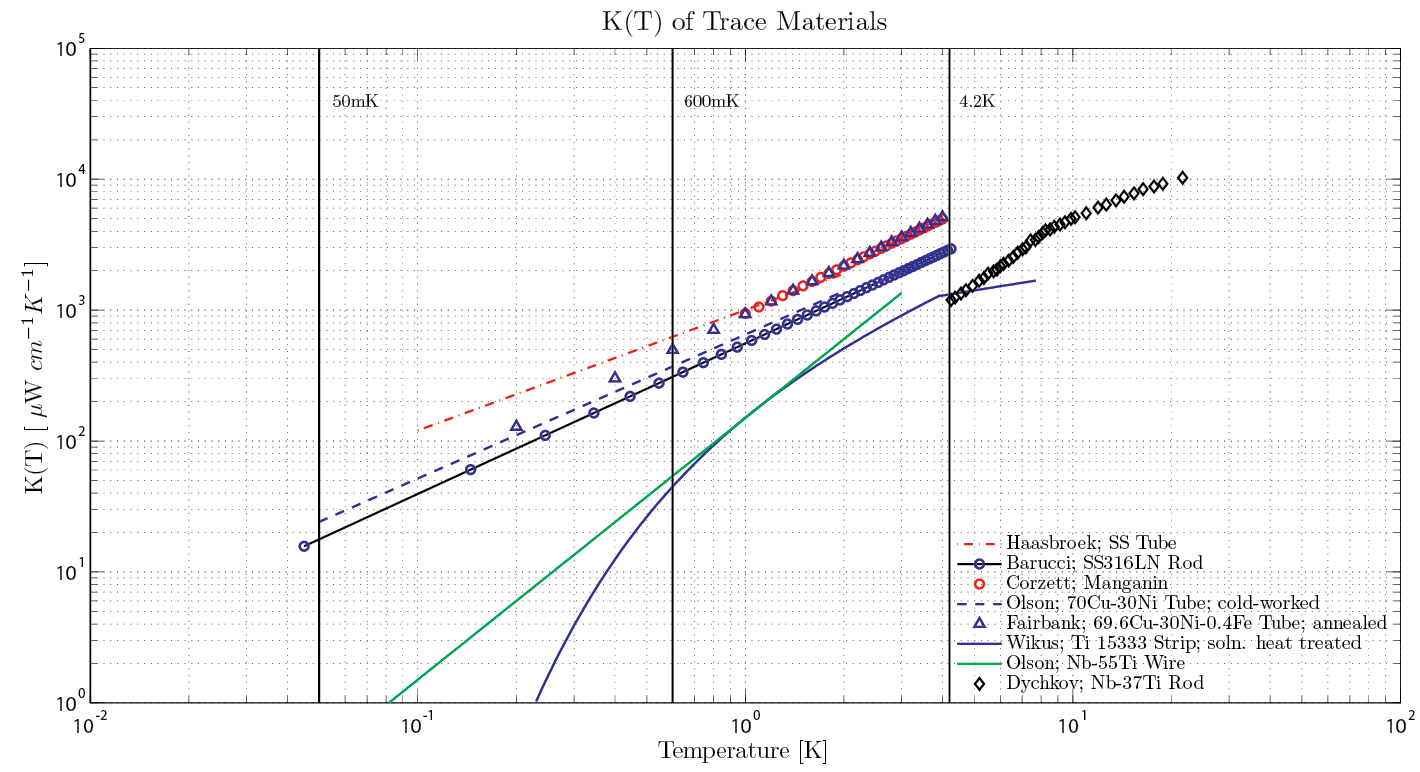
\includegraphics[width = .8\textwidth]{Trace_material_k.png}
\caption{Thermal conductivities for trace materials. High and low values were taken from the literature when a significant variation was present among data. Data from: Haasbroek \cite{has}, Barucci \cite{Barucci2008}, Corzett{cor}, Olson \cite{ols}, Fairbank \cite{fair}, Wikus \cite{wik}, Dyachkov \cite{dya}.}
\end{figure}


\subsection{Resistivities of Trace Materials}
Since Ti15-3 has a transition temperature of 3.9K (as measured at MIT), it will not be in a superconducting state throughout the 4.2K - 600mK span. However, as long as the resistivity remains low, it can still be used. Table 2 presents the resistivity as compared to other possible trace materials.

\begin{table}[h]
\centering
\begin{threeparttable}
\begin{tabular}{l|c|c|c|c}
Alloy & \multicolumn{3}{c}{Resistivity in $\mu$ $\Omega$ $cm$} \\\toprule
 & 300K & 273K & 10K & 4.2K \\\midrule
70Cu-30Ni & - & 38.4 & - & 36.4 \\
Constantan & 49.1 & - & 46.1 & - \\
Manganin (4\%Ni) & 47.6 & - & 41.9 & - \\
Ti15-3 & 146 & - & - & 173 \\
SS316 & - & 76.5 & - & 55.3 \\
50Nb-50Ti & 76.7 & - & 54 & 0 \\
\end{tabular}
\end{threeparttable}
\caption{Resistivities of possible trace materials.}
\end{table}

Though the resistivity of Ti15-3 is higher than other candidate materials, if we consider a trace 10 mils wide and 1 mil thick, we get a resistance of
$$
\frac{R}{Length} = \frac{173 \cdot 10^{-6} \Omega cm}{6.45 \cdot 10^{-5} cm^{2}} = 2.68 \Omega / cm
$$

\subsection{Phonon Transmission Line Dimensions}

The new proposed dimensions for the phonon transmission line are shown below. The total widths of the lines (as given below) are larger than previously thought, which may alter design considerations. The trace separation is 10 mil between every trace, regardless of width. Though this places adjacent traces near one another, by alternating trace types as shown in Figures 3,4, and 5, we can increase the spacing between the lines whose cross-talk we are concerned with.

\begin{itemize}
\item 4.2K to 600mK
    \begin{itemize}
    \item 4.2K-600mK cable length = 9.24cm
    \item Trace width = 10 mil
    \item Total traces = $2\cdot12$ QET Bias Resistor + $2\cdot12$ SQUID Bias + $2\cdot12$ SQUID Feedback + $2\cdot6$ LED + $2\cdot4$ Charge Readout Bias + $2\cdot4$ Charge Feedback = 100 Traces
    \item Horizontal trace separation = 10 mil
    \item Trace thickness = 0.8 mil
    \item Total line width = 1.01 inches
    \item Total trace cross-section = 0.0052 $cm^2$
    \item Total Kapton cross-section = 0.0098 $cm^2$
    \item Total adhesive cross-section = 0.0130 $cm^2$
    \end{itemize}
\item 600mK to 50mK
    \begin{itemize}
    \item 600mK-50mK cable length = 5.04cm
    \item Trace width:
        \begin{itemize}
        \item QET Signal = 40 mil
        \item QET Bias Resistor, LED line, Thermometry line, Charge readout = 10 mil
        \end{itemize}
    \item Total traces = $2\cdot12$ QET Signal + $2\cdot12$ QET Bias Resistor + $2\cdot6$ LED + $2\cdot4$ Charge Readout Bias + $2\cdot4$ Charge Feedback = 76 Traces
    \item Horizontal trace separation = 10 mil
    \item Trace thickness = 0.8 mil
    \item Total line width = 1.13 inches
    \item Total trace cross-section = 0.0076 $cm^2$
    \item Total Kapton cross-section = 0.0109 $cm^2$
    \item Total adhesive cross-section = 0.0146 $cm^2$
    \end{itemize}
\end{itemize}

\newpage

\begin{figure}[h]
\centering
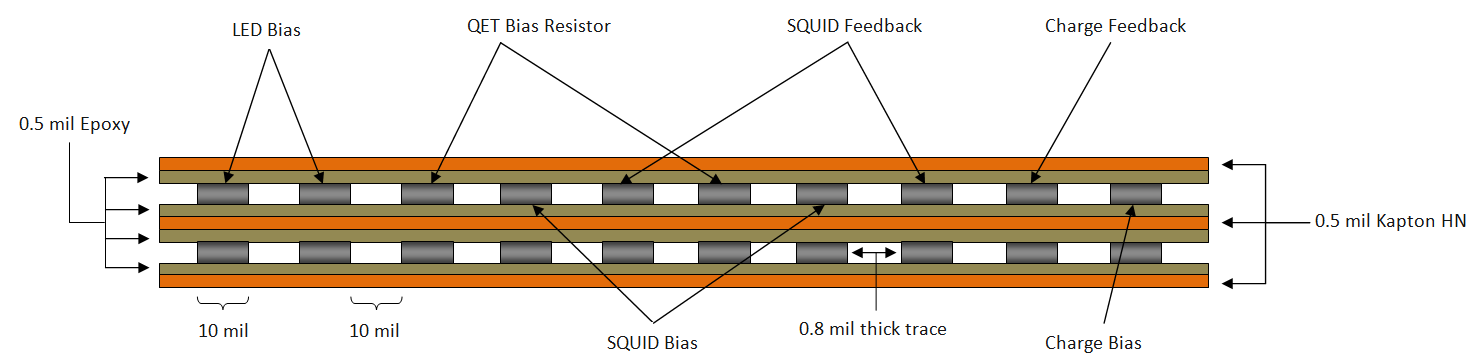
\includegraphics[width = .9\textwidth]{4K_600mK_diagram.png}
\caption{Cross-section for 4K-600mK phonon transmission line showing 20 of the 100 traces.}
\end{figure}
~\\
~\\
\begin{figure}[h]
\centering
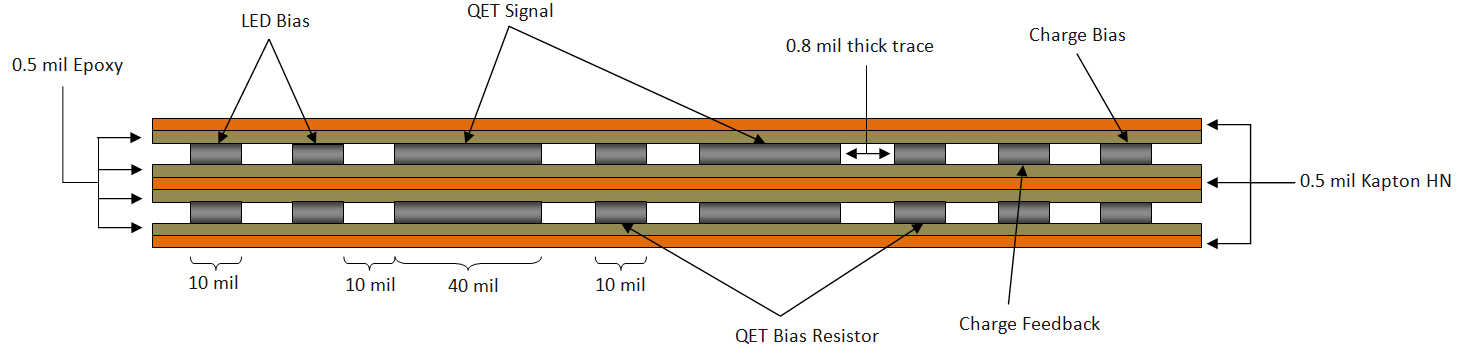
\includegraphics[width = .9\textwidth]{600mK_50mK_diagram.png}
\caption{Cross-section for the 600mK-50mK section of the phonon transmission line showing 16 of the 76 traces.}
\end{figure}
~\\
~\\
\begin{figure}[h]
\centering
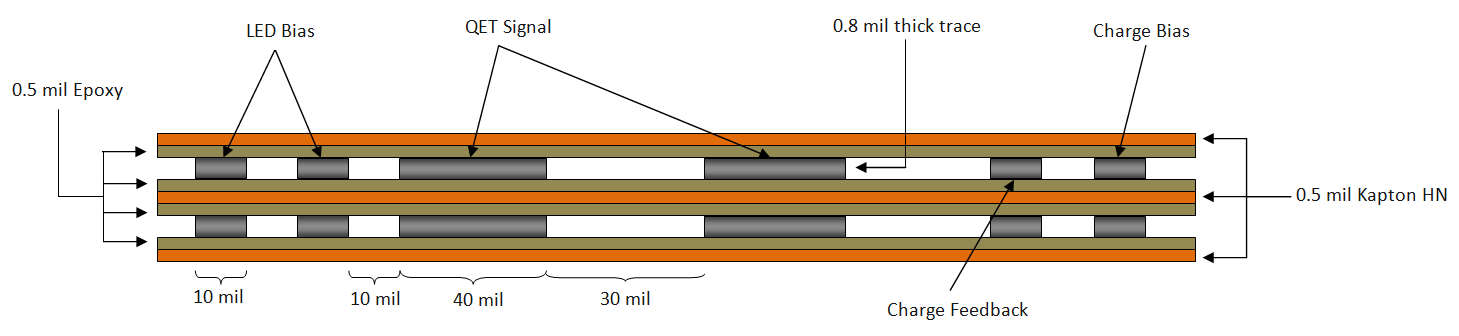
\includegraphics[width = .9\textwidth]{50mK_10mK_diagram.png}
\caption{Cross-section for the 50mK-10mK section of the phonon transmission line showing 12 of the 52 traces.}
\end{figure}

\newpage

\begin{itemize}
\item 50mK to 10mK
    \begin{itemize}
    \item 50mK-10mK cable length = 3.25cm
    \item Trace width:
        \begin{itemize}
        \item QET Signal = 40 mil
        \item LED line, Thermometry line, Charge readout = 10 mil
        \end{itemize}
    \item Total traces = $2\cdot12$ QET Signal + $2\cdot6$ LED + $2\cdot4$ Charge Readout Bias + $2\cdot4$ Charge Feedback = 52 Traces
    \item Horizontal trace separation = 30 mil between QET ; 10 mil between all else
    \item Trace thickness = 0.8 mil
    \item Total line width = 1.13 inches
    \item Total trace cross-section = 0.0064 $cm^2$
    \item Total Kapton cross-section = 0.0109 $cm^2$
    \item Total adhesive cross-section = 0.0146 $cm^2$
    \end{itemize}
\end{itemize}

\subsection{Phonon Transmission Line Heat Load}

The heat loads for the Phonon line using different trace materials are shown below \footnotemark. As you can see, the heat load from the traces is significant, especially for the 4.2K-600mK span.
The 50mK-10mK span assumes placement of a heat sink at the detector end of the tower (before the copper tube which holds the detector housings) which shortens the 50mK-10mK cable length to only 3.25cm. If we were to create a heat sink closer to the detectors, this could be significantly reduced.

\begin{table}[h]
\begin{threeparttable}
\begin{tabular}{rrrr|rrr}
\toprule
 & \multicolumn{6}{c}{Heat Load for 48 Towers in $\mu$W} \\
  & 5K-1K & 1K-100mK & 100mK-40mK & 4.2K-600mK & 600mK-50mK & 50mK-10mK \\
 \cmidrule(r){2-7}
   Ti15-3 \cite{wik} & 590.6 & 20.20 & $1.0\cdot10^{-4}$ & 412.5 & 2.93 & $1.1 \cdot 10^{-6}$ \\
   45Nb-Ti \cite{ols} & 1047 & 22.89 & 0.0279 & 623.9 & 4.95 & 0.0037 \\
   Manganin (2\%Ni) \cite{Peroni1999} & 2476 & 192.9 & 1.321 & 1707 & 62.19 & 0.317 \\
   SS316 \cite{lou} \cite{Barucci2008} & 1347 - 1846  & 117.7 - 235.8 & 0.938 - 3.087 & 941.1 - 1351 & 39.33 - 88.76 & 0.238 - 0.9405 \\
   70Cu-30Ni \cite{pob} \cite{ols} & 1483 - 2480 & 140.7 - 190 & 1.25 - 1.273 & 1047 - 1706 & 48.26 - 60.94 & 0.303 - 0.330 \\
   Al5056 \cite{Coccia1983} & 3.98E+5 & 2273 & .4225 & 2.05E+5 & 321.1 & 0.031 \\
   Kapton \cite{bar} & 237.6 & 20.11 & 0.265 & 171.1 & 7.26 & 0.076 \\
   Epoxy Adhesive &&&&&& \\
   \multicolumn{2}{c}{\bf{Total Phonon Line}} & & & & & \\
   with Ti15-3 & 828.3 & 40.31 & 0.265 & 583.6 & 10.19 & 0.076 \\
   with 45Nb-Ti & 1285 & 43.00 & 0.292 & 795 & 12.21 & 0.0793 \\
   with Manganin & 2714 & 213 & 1.585 & 1878 & 69.45 & 0.3925 \\
   with SS316 & 1584 - 2083 & 137.8 - 255.9 & 1.203 - 3.351 & 1112 - 1522 & 46.59 - 96.02 & 0.314 - 1.016 \\
   with 70Cu-30Ni & 1721 - 2717 & 160.8 - 210.1 & 1.515 - 1.537 & 1218 - 1877 & 55.52 - 68.2 & 0.3787 - 0.406 \\
   with Al5056 & 3.99E+5 & 2293 & 0.687 & 2.05E+5 & 328.1 & .106 \\
  \bottomrule
\end{tabular}
\end{threeparttable}
\caption{Heat loads for constituents of the phonon cable as well as the total cable heat load for various materials for a total of 48 towers. Assumes all trace thicknesses are 0.84 mils. The large heat load at the 50mK-10mK span for the phonon cable is due to short cable length (3.25cm) created by placing a heat sink at the bottom of the tower.}
\end{table}

\footnotetext{Constantan (55Cu-45Ni) was considered as an alternative to Cupro-Nickel, due to its lower Copper content. However, it was found \cite{tou} to have a higher thermal conductivity than 70Cu-30Ni.}

\newpage
\subsection{Sonnet Modeling for Phonon Line}
Between the SQUIDS and our detectors, we have set an inductance limit of roughly 30nH between signal/return lines. To ensure that our cable would meet this requirement, Sonnet modeling software was used to simulate the line with 40mil wide, 0.8mil thick traces at a center-to-center separation of 2.3mil. This yields:
$$
L = 22.4\frac{nH}{20"}
$$
as well as,
$$
C = 471\frac{pF}{20"}
$$
for capacitance between the lines.

\section{Charge Readout Lines}

The form of the future charge readout lines is still under debate. Since noise is only a concern on the gate wires, the charge feedback and bias pairs can be integrated into the flexible parallel-trace transmission line design. The 4 remaining gate wires have a few available options. The simplest option would be for the lines to remain vacuum coaxes. The next option involves a flexible coaxial cable produced by AXON' The last option would be to make our own cable with low noise properties.

If we keep the vacuum coaxes, we will alter the design slightly to allow removal of the coaxes from the tower. This would involve a type of carbon fiber rod supported frame to which the wires are mounted, as depicted in Figure 6. Though this could be a low heat load design, it is the least convenient option. Heat loads are presented in Table 4. The wires would be the same 1.2 mil diameter NbTi lines currently used in our towers, however would have an additional heat sink at the newly available externalized 50mK stage on the next generation tower design. We see that the heat loads for this option are rather large, due to the carbon fiber rods. While the calculations have assumed a 40mil rod thickness, our supplier for rods also has 33mil, 30mil, 20mil, and 10mil diameter rod options, which could reduce heat loads.

The next option involves a coaxial cable from AXON' \footnotemark.
\footnotetext{Another company, Texcal, was considered, as they also produce low-noise cabling. Unfortunately, their cables use silver-plated copper conductors, whose thermal conductivity far exceeds what is acceptable for our purposes.}
This cable uses Constantan as a conductor material, PTFE for a housing, and Celloflan dielectric (porous PTFE); The cable's cross-section is shown in Figure 6. A thin graphite coating on the outside of the Celloflan dielectric prevents static charge build-up on the insulator -- our main source of noise in the gate wires. The suitability of this option depends on expected heat loads from the cable. These are shown in Table 4. The calculations use Cupro-Nickel (70Cu-30Ni) thermal conductivity in place of Constantan \footnotemark, as well as simple PTFE in place of Celloflan. The high expected heat loads from this cable will likely rule it out as a candidate for replacing the vacuum coax design.

\footnotetext{It was found that the actual thermal conductivity of Constantan is slightly higher than Cupro-Nickel, but is close enough for approximation purposes. If this is considered a viable option, more accurate calculations will be done.}
Another option is to simply alter a cable to have low-noise characteristics. This could be made possible with a flexible polyimide cable whose dielectric has undergone ion implantation to increase the conductivity to near that of graphite \footnotemark. This would serve the same function as the graphite layer in the AXON' coaxial cable -- preventing static charge build-up. Heat loads for this option are not presented, as the potential form of these cables is as-of-yet unknown.

\footnotetext{See, for instance, \cite{Chen2009}}

\begin{figure}[h]
$\vcenter{\hbox{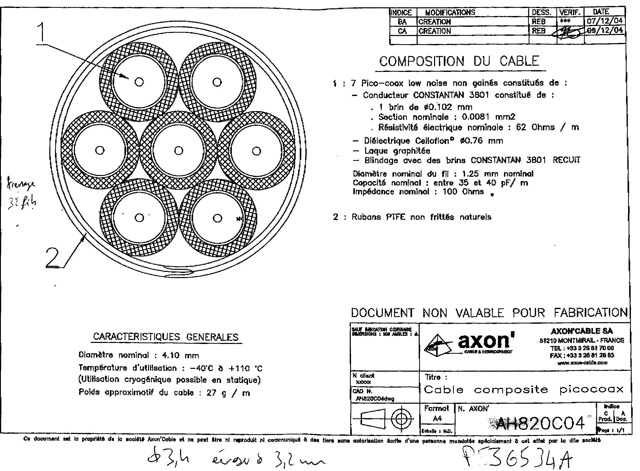
\includegraphics[width = .5\textwidth]{Edelweiss_cable.jpeg}}}$
$\vcenter{\hbox{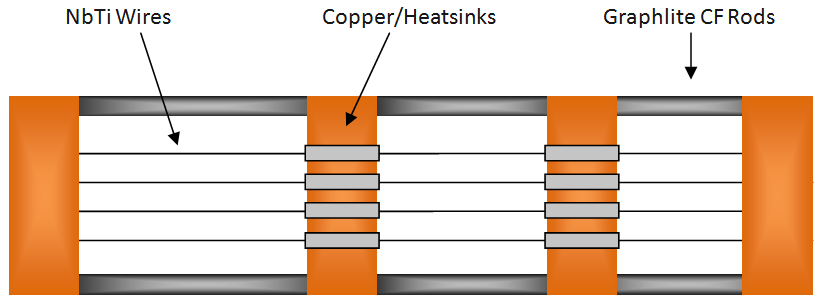
\includegraphics[width = .5\textwidth]{Charge_vacuum_design.png}}}$
\caption{Two possible designs for future charge gate wires. Left is the specially made AXON' cable (to have a Conastantan conductor). Right shows the basic structure of a removable vacuum coax design with copper heatsink connections supported by carbon fiber rods.}
\end{figure}

\subsection{Charge Readout Heat Loads}

The total charge readout line heat load contribution for a 12 tower experiment is presented below in Table 4. These calculations assume 4 gate wires per detector, so 288 wires for 12 towers (or 288 coaxes in the case of the AXON' cable).

\begin{table}[h]
\begin{threeparttable}
\begin{tabular}{rrrr|rrr}
\toprule
 & \multicolumn{6}{c}{Charge Coax Heat Loads for 12 Towers in $\mu$W} \\
  & 5K-1K & 1K-100mK & 100mK-40mK & 4.2K-600mK & 600mK-50mK & 50mK-10mK \\
 \cmidrule(r){2-7}
   Vacuum Coax Design & 122.3 & 16.34 & 0.135 & 94.3 & 5.17 & 0.031 \\
   AXON' Cable & 2736 - 4439 & 261.56 - 351.22 & 3.163 - 3.221 & 1862 - 2988 & 88.59 - 110.91 & 0.768 - 0.827 \\
  \bottomrule
\end{tabular}
\end{threeparttable}
\caption{Heat loads for charge readout coaxes for 12 towers. With 50mK heat sinking, assumes cable lengths of: 4.2K - 600mK = 7.8cm ; 600mK - 50mK = 2.7cm ; 50mK - 10mK = 1.5cm. Assumes 4 lines (or coaxes) per detector, 6 detectors per tower. The vacuum coax calculations assume two 40 mil diameter rods between each stage, which constitute the frame for the removable vacuum coaxes. These dominate the heat loads ($>95\%$).}
\end{table}

\section{Wiring for 300K - 4.2K}

We must design cable to run from room temperature (300K) to the HEMTs on the tower (4.2K). This cable must meet resistance, thermal, and practical requirements. The upper limit on round trip resistance for the lines is around 200$\Omega$, while the upper limit for heat load is 500mW on 4.2K. Apart from these considerations, the cable must be thin enough to be flexible, the dimensions work-able, and the traces should be solderable\footnotemark.

To meet the heat load restrictions of the cable, a 77K heat sink will be placed along the cable. This will be located around 20" down the cable from room temperature. From here, the 77K - 4.2K length will run around 90" until the 4.2K heat sink. From here, there will be 20" to the HEMTs at the tower. 500mW is a larger heat load than we expect from any reasonably designed cable, so minimizing heat load is not the primary design consideration.

\footnotetext{OFHC Copper was considered as an option, as it is the easiest to solder and has a much smaller resistivity, but the thermal conductivity was nearly 5 orders of magnitude higher than the range of materials in Figure 7. Dimensions could not be decreased enough to produce a viable heat load.}

The resistivity of some of the candidate materials is shown in Table 2. This will set a limit on the minimum dimensions of the traces to keep below 200$\Omega$ for the lines. This, as well as the ease with which the traces can be manufactured into a cable (ability to solder to the traces, flexibility, strength, availability) is the main consideration for selection of dimensions and trace material.

\begin{SCfigure}
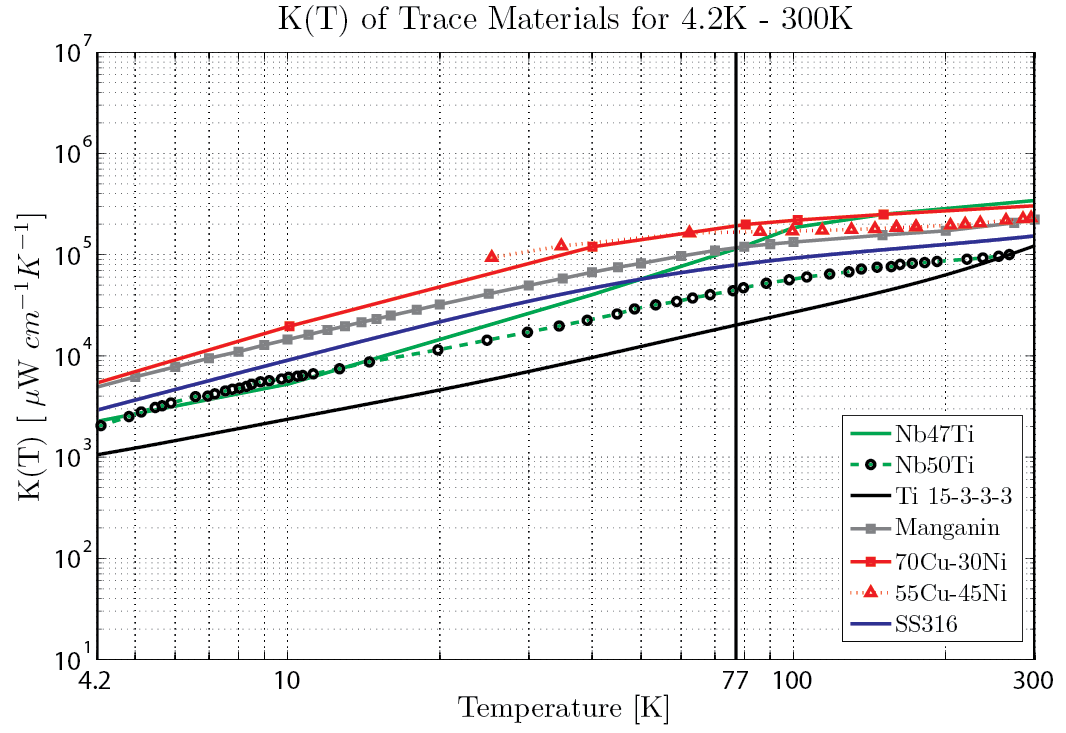
\includegraphics[width = .65\textwidth]{Trace_matl_300K.png}
\caption{Thermal conductivities of viable trace materials for a cable spanning 4.2K to 300K. References for data are: \newline Nb47Ti - Tekdata website ; Nb50Ti - Flachbart \cite{Flachbart1978} ; Ti 15333 - Wikus \cite{wik} ; Manganin (84Cu-4Ni-12Mn) - Touloukian \cite{tou} ; 70Cu-30Ni - Tekdata website ; 55Cu-45Ni - Touloukian \cite{tou} ; SS316 - NIST database.}
\end{SCfigure}

\subsection{Expected Heat Loads}

The predicted heat loads for some of the candidate materials on the 77K stage and 4.2K stage are presented in Table 5. These heat loads assume the cross-sections presented for each material in the same table. Cross-sections for each material were minimized based on each material's resistivity to produce a line resistance of 200$\Omega$. As the resistivity of each material varies with temperature, the maximum value of resistivity from Table 2 was assumed for each material across the temperature range to provide a safety buffer in resistance.

The heat loads are all relatively similar despite very different thermal conductivities, due to the different minimum cross-sections. After factoring in resistance, the advantage of Ti15-3-3-3 over 70Cu-30Ni is only a factor of 2 for power onto 4.2K, despite Ti15-3-3-3 being about a factor of ten better in thermal conductivity.

Considering the difficulty in fabricating a cable out of Ti15-3-3-3, and the large dimensions that would be required for a Ti15-3-3-3 trace (30 mil wide traces would still have to be 7.5 mils thick) it is not the best option. Instead, Manganin or 70Cu-30Ni are recommended.

\begin{table}[h]
\centering
\begin{threeparttable}
\begin{tabular}{l|ccc}
\toprule
Material & $A_{min}$ [$cm^2$] & Power to 77K [$\mu W$] & Power to 4.2K [$\mu W$] \\
\midrule
70Cu-30Ni & 1.2680E-4 & 1.301E+7 & 3.802E+5 \\
Ti15-3-3-3 & 5.7125E-4 & 1.374E+7 & 1.605E+5 \\
Manganin (4\%Ni) & 1.5718E-4 & 1.0220E+7 & 2.862E+5 \\
SS316 & 2.526E-4 & 1.187E+7 & 3.180E+5 \\
\bottomrule
\end{tabular}
\end{threeparttable}
\caption{Minimum cross-sections and expected heat loads for candidate materials for a 48-tower experiment. Minimum cross-sections are calculated from the maximum resistivities of each material in Table 2 and used to calculate heat loads.  Only some of the candidate materials are presented for comparison, as heat loads are not a major concern.}
\end{table}


\section{Tower Thermal Stand-offs}
Unlike the wiring, the thermal stand-offs for the tower can be made out of a multitude of materials. Both tube and hexa-pod structures have been proposed for these materials. These candidates are evaluated based on their thermal conductivity and their strength (which allows us to decrease their cross-sectional area).

\subsection{Thermal Conductivities of Tower Materials}
In SuperCDMS, the dominant heat load came from the thermal stand-offs, so replacement materials aim for a significant improvement in thermal power conducted between stages. Figure 8 shows the candidate materials for thermal stand-offs based on radioactivity screening acceptability. Though the Graphlite rods are much higher in thermal conductivity, their strength makes them a viable material.

\begin{figure}
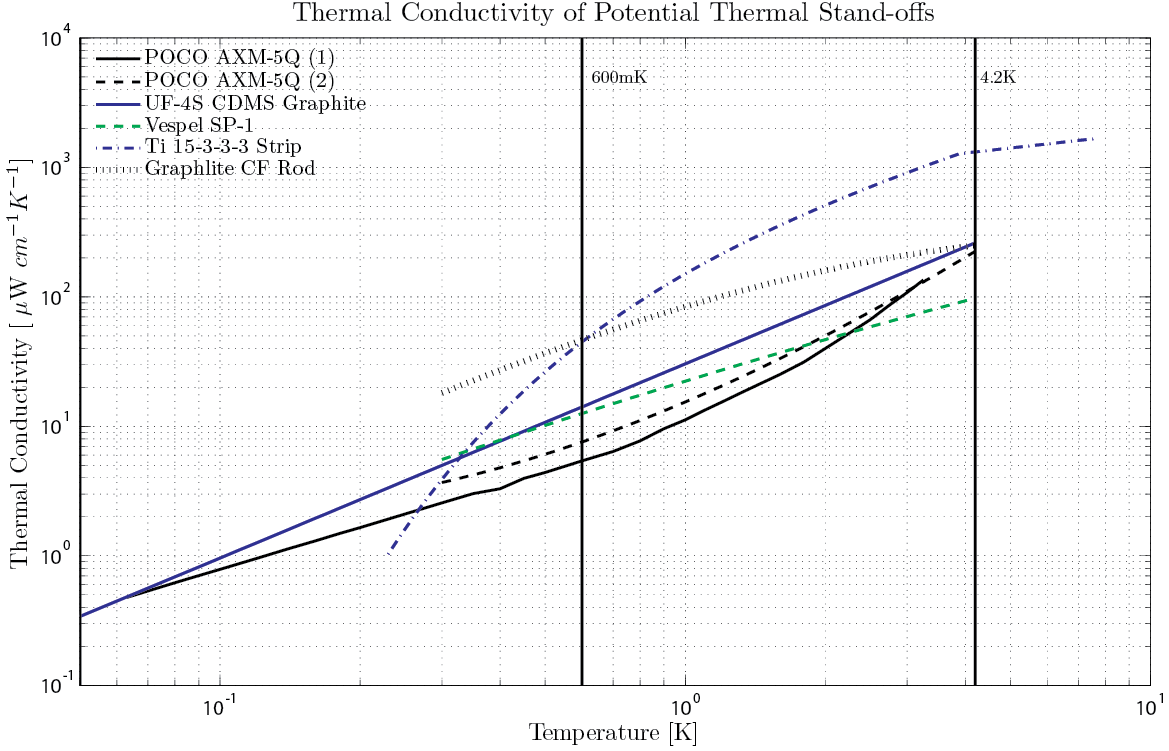
\includegraphics[width = \textwidth]{Stand_off_graph.png}
\caption{Thermal conductivities of candidate thermal standoff materials. POCO AXM-5Q (1) is from Woodcraft \cite{woo:gr} , while POCO AXM-5Q (2) was measured by Marc Runyan at Caltech \cite{run}.}
\end{figure}

\subsection{Stand-off Configurations}
There are currently two possibilities for the thermal stand-off configuration. The first is a hexapod structure, while the second is a thin walled tube.

The hexapod structure allows us to limit power loads by angling the stand-off material, which increases the effective length of the material. In addition, it limits cross-sections, as it is a very open structure. This has only been proposed for the Graplite rods so far, but could conceivably be applied to the Vespel or Ti15-3 as well.

The other materials were designed to be thin walled tubes. The dimensions of the tubes were optimized using the analytical model given in my earlier report. Using a given tube length, radius and thickness are optimized to minimize cross-section while maintaining a failure limit of 130 lbs (59 kg). This limit is in shear loading of the tower (mimicking holding the tower sideways with the detectors attached). The detectors themselves will weigh 1.4 kg apiece. With 6 detectors that is around 10 kg. We will need to figure out the equivalent load at the end of the tube to see if this results in greater than 130 lbs.

\subsection{Stand-off Heat Loads}

The stand-off lengths used to calculate heat loads were chosen to be: 4.2K-600mK = 1.68 inches ; 600mK-50mK = 1.65 inches ; 50mK-10mK = 1.30 inches. These can easily be adjusted depending on heat load constraints. The heat loads for materials of various dimensions were calculated for each stage. At each stage, the heat load for CF Graphlite rods was calculated, based on dimensions suggested by Marc Runyan. In addition, several thin-wall tube candidates are presented. The heat load for optimized dimensions are given, as well as "safer" dimensions (larger  radius and/or thickness).

\begin{table}[h]
\begin{small}
\begin{threeparttable}
\begin{tabular}{lrrrrl}
  \multicolumn{5}{l}{{\Large 4.2K - 600mK: Thermal Stand-off Heat Loads in $\mu$W, 12 Towers}} \\
\toprule
\bf{{\large Material}}& \multicolumn{2}{c}{145lb. Failure} & \multicolumn{2}{c}{290lb. Failure} & Ref.\\
\cmidrule(r){2-5}
& 5K - 1K & 4.2K - 600mK & 5K - 1K & 4.2K - 600mK & \\
Current CDMS Graphite; $(2"\oslash,0.028")$  & 3708 & 2424 & 3708 & 2424 & \cite{lem}\\
6 Graphlite CF Rods; ($0.08" \oslash$ @ $45^{o}$) & 308.4 & 238.8 & 308.4 & 238.8 & \cite{run}\\
Vespel SCP-5000; $(0.74"\oslash,0.024")|(0.94"\oslash,0.030")$ & 282.6\tnote{\dag} & 203.5\tnote{\dag} & 448.4\tnote{\dag} & 322.9\tnote{\dag} & \cite{run}\\
Vespel SP-1; $(.96"\oslash,0.027")|(1.2"\oslash,0.0347")$ & 412.7 & 297.1 & 662.6 & 477.2 & \cite{run}\\
POCO-AXM 5Q; $(1.86"\oslash,0.013")|(2.28"\oslash,0.0172")$ & (900,721) & (446,425) & (1467,1175) & (726,693) & \cite{woo:gr},\cite{run}\\
Ti 15-3-3-3 $(0.66"\oslash,0.0055")|(0.82"\oslash,0.0072")$ & 720.5 & 503.2 & 1168.3 & 816.0 & \cite{wik}\\
\bottomrule
\end{tabular}
\begin{tablenotes}
\item[\dag] Note that the integrated thermal conductivity of Vespel SP-1 was used as a proxy for
    SCP-5000.
\end{tablenotes}
\end{threeparttable}
\caption{Heat loads for 4.2K-600mK stage including non-ideal fridge temperatures. Structures designed for both 145lb. and 290lb. failure limits. Dimensions are given in (diameter, thickness) pairs for tubes. The left and right set correspond to 145lb. and 290lb. failure limits respectively. The CF Graphlite supports are rods with the given dimensions. Varying POCO heat loads come from the two referenced data. Stage length is 1.68 inches.}
\end{small}
\end{table}

\begin{table}[h]
\begin{small}
\begin{threeparttable}
\begin{tabular}{lrrrr}
  \multicolumn{5}{l}{{\Large 600mK - 50mK: Thermal Stand-off Heat Loads in $\mu$W, 12 Towers}} \\
\toprule
\bf{{\large Material}}& \multicolumn{2}{c}{145lb. Failure} & \multicolumn{2}{c}{290lb. Failure} \\
\cmidrule(r){2-5}
& 1K - 100mK & 600mK - 50mK & 1K - 100mK & 600mK - 50mK \\
Current CDMS Graphite; $(2"\oslash,0.028")$  & 40.8 & 11.4 & 40.8 & 11.4\\
6 Graphlite CF Rods; ($0.08" \oslash$ @ $45^{o}$) & 15.0 & 4.8 & 15.0 & 4.8 \\
Vespel SCP-5000; $(0.74"\oslash,0.024")|(0.94"\oslash,0.030")$ & 10.5\tnote{\dag} & 3.5\tnote{\dag} & 16.8\tnote{\dag} & 5.6\tnote{\dag} \\
Vespel SP-1; $(.96"\oslash,.027")|(1.18"\oslash,0.035")$ & 15.4 & 5.2 & 24.8 & 8.3 \\
POCO-AXM 5Q; $(1.84"\oslash,.013")|(2.26"\oslash,0.0172")$ & (6.6,9.1) & (2.1,3.0) & (10.7,14.9) & (3.4,4.8) \\
Ti 15-3-3-3 $(0.66"\oslash,.0054")|(0.82"\oslash,0.0071")$ & 9.1\tnote{\S} & 1.3\tnote{\S} & 14.9\tnote{\S} & 2.2\tnote{\S} \\
\bottomrule
\end{tabular}
\begin{tablenotes}
\item[\dag] Note that the integrated thermal conductivity of Vespel SP-1 was used as a proxy for SCP-5000.
\end{tablenotes}
\end{threeparttable}
\caption{Heat loads for 600mK - 50mK stage including non-ideal fridge temperatures. Structures designed for both 145lb. and 290lb. failure limits. Dimensions are given in (diameter, thickness) pairs for tubes. The left and right set correspond to 145lb. and 290lb. failure limits respectively. The CF Graphlite supports are rods with the given dimensions. Stage length is 1.65 inches. References for data are the same as in Table 5.}
\end{small}
\end{table}

\begin{table}[h]
\begin{small}
\begin{threeparttable}
\begin{tabular}{lrrrr}
  \multicolumn{5}{l}{{\Large 50mK - 10mK: Thermal Stand-off Heat Loads in $\mu$W, 12 Towers}} \\
\toprule
\bf{{\large Material}}& \multicolumn{2}{c}{145lb. Failure} & \multicolumn{2}{c}{290lb. Failure} \\
\cmidrule(r){2-5}
& 100mK-40mK & 50mK - 10mK & 100mK - 40mK & 50mK - 10mK \\
Current CDMS Graphite; $(2"\oslash,0.028")$  & 1.368E-1 & 2.64E-2 & 1.368E-1 & 2.64E-2\\
6 Graphlite CF Rods; ($0.08" \oslash$ @ $45^{o}$) & 8.64E-2 & 2.04E-2 & 8.64E-2 & 2.04E-2 \\
Vespel SCP-5000; $(0.68"\oslash,0.022")|(0.86"\oslash,0.028")$ & 6.83E-2\tnote{\dag} & 1.72E-2\tnote{\dag} & 1.084E-1\tnote{\dag} & 2.74E-2\tnote{\dag} \\
Vespel SP-1; $(.88"\oslash,.025")|(1.08"\oslash,0.033")$ & 1.002E-1 & 2.53E-2 & 1.637E-1 & 4.13E-2 \\
POCO-AXM 5Q; $(1.66"\oslash,.013")|(2.02"\oslash,0.017")$ & (4.9E-2,6.0E-2) & (1.3E-2,1.5E-2) & (8.0E-2,9.8E-2) & (2.2E-2,2.4E-2) \\
Ti 15-3-3-3 $(0.60"\oslash,.0052")|(0.74"\oslash,0.0068")$ & 3.8E-5\tnote{\S} & 4.4E-7\tnote{\S} & 6.3E-5\tnote{\S} & 7.2E-7\tnote{\S} \\
\bottomrule
\end{tabular}
\begin{tablenotes}
\item[\dag] Note that the integrated thermal conductivity of Vespel SP-1 was used as a proxy for SCP-5000.
\item[\S] The exponent for thermal conductivity of Ti 15-3-3-3 was fixed at 230mK -- the end of the data range -- and extrapolated to 10mK. The low temperature thermal conductivity will be verified through tests.
\end{tablenotes}
\end{threeparttable}
\caption{Heat loads for 50mK-10mK stage including non-ideal fridge temperatures. Structures designed for both 145lb. and 290lb. failure limits. Dimensions are given in (diameter, thickness) pairs for tubes. The left and right set correspond to 145lb. and 290lb. failure limits respectively. The CF Graphlite supports are rods with the given dimensions. Stage length is 1.3 inches. References for the data are the same as in Table 5.}
\end{small}
\end{table}

One can see from the tables that there are still many choices to be made with respect to the thermal stand-offs. We will likely make some test pieces to then test mechanically before any final decisions are made.

\newpage
\section{Total Heat Loads for 12 Tower Experiment}
\begin{table}[h]
\begin{threeparttable}
\begin{tabular}{rrrr|rrr}
\toprule
 & \multicolumn{6}{c}{Contributions \& Total Heat Loads per Tower in $\mu$W} \\
  & 1K & 100mK & 40mK & 600mK & 50mK & 10mK \\
 \cmidrule(r){2-7}
   Phonon Line & 19.6 & 1.20 & $11.0 \cdot 10^{-3}$  & 13.9 & 0.355 & $3.2 \cdot 10^{-3}$ \\
   Charge Line & 0.4 & 0.01 & $1.6 \cdot 10^{-5} $ & 0.3 & 0.002  & $2.2 \cdot 10^{-6}$ \\
   Stand-offs & 25.7 & 0.97 & $7.2 \cdot 10^{-3}$ & 19.9 & 0.340 & $1.7 \cdot 10^{-3}$ \\
   SQUID Dissipation & 5.8 & NA & NA & 5.8 & NA & NA \\
   SQUID Shunt R & NA & 0.50 & NA & NA & 0.500 & NA \\
   \bf{Total Power (1 Tower)} & \bf{51.5} & \bf{2.68} & $ \bf{18.2 \cdot 10^{-3}}$ & \bf{39.8} & \bf{1.20} & $\bf{4.9 \cdot 10^{-3}}$ \\
  \bottomrule
\end{tabular}
\end{threeparttable}
\caption{Heat load contributions and total heat load for 1 tower. Powers given are those dissipated at the temperature stage indicated. Assumes dimensions stated in previous sections. CF was used instead of Ti15-3 in the lowest stage in order to be conservative. However, we predict that the heat load to 10mK can be much lower than these numbers by using Ti15-3 stand-offs. Heat loads for the charge readout cable assume 50mK heat-sinking. We could budget for avoiding a 50mK heat sink by using Ti15-3 stand-offs, which will likely have much lower heat loads to base. }
\end{table}

\begin{table}[h]
\begin{threeparttable}
\begin{tabular}{rrrr|rrr}
\toprule
 & \multicolumn{6}{c}{\large{Total Power for 12 Tower Set-up in $\mu$W}} \\
  & 1K & 100mK & 40mK & 600mK & 50mK & 10mK \\
 \cmidrule(r){2-7}
   \bf{\large{Power}} & \large{\bf{618.0}} & \large{\bf{32.16}} & \large{\bf{0.218}} & \large{\bf{477.6}} & \large{\bf{14.40}} & \large{\bf{0.059}} \\
\bottomrule
\end{tabular}
\end{threeparttable}
\caption{Heat loads for a 12-tower experiment. Heat loads to base will likely be lower if Ti15-3 is used as a stand-off.}
\end{table}


\newgeometry{hmargin = 1.8cm,vmargin = 2cm}
\newpage

\appendix
\section{Thermal Conductivity Variation of Trace Materials}

\begin{figure}[h]
\begin{centering}
\subfloat[]
    {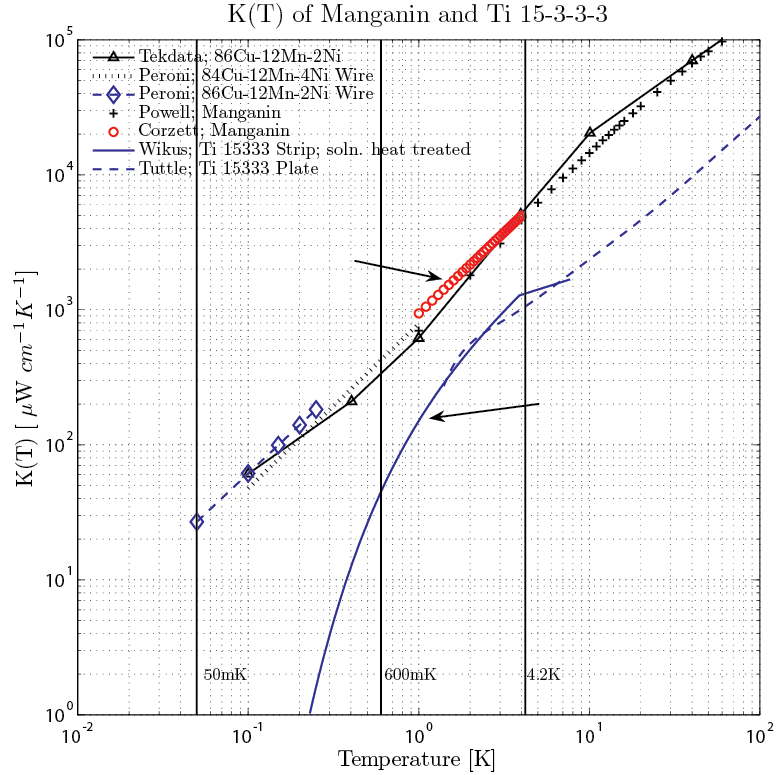
\includegraphics[width=0.41\textwidth]{Mang_Ti_graph.png}}
\subfloat[]
    {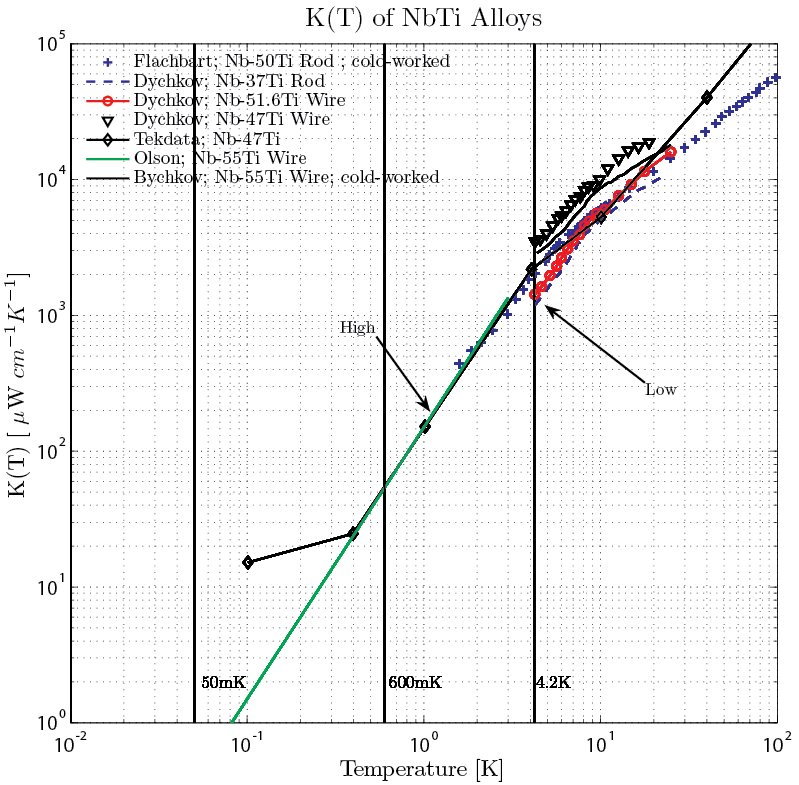
\includegraphics[width=0.41\textwidth]{NbTi_graph.png}}

\subfloat[]
    {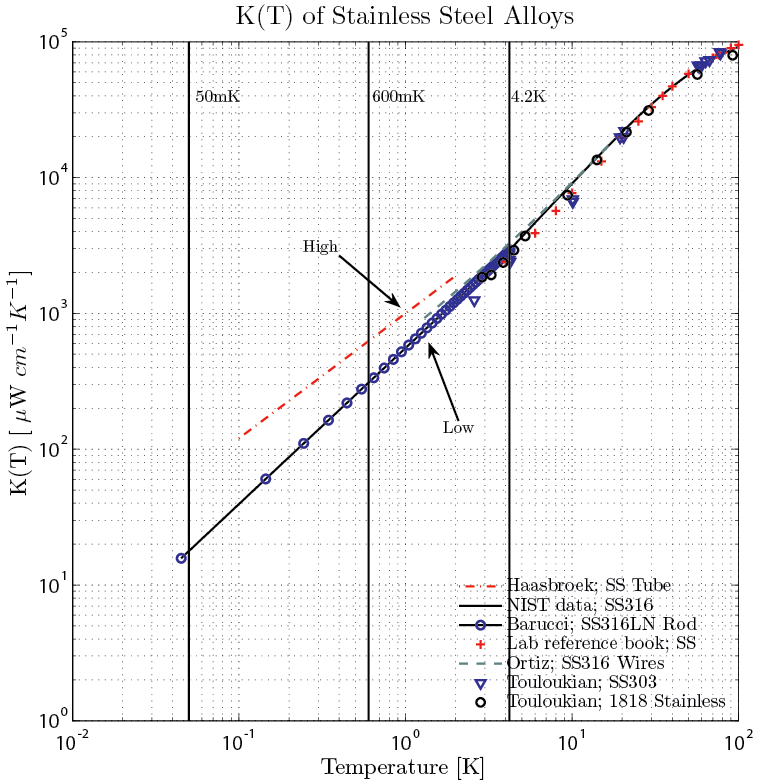
\includegraphics[width = 0.41\textwidth]{SS_graph.png}}
\subfloat[]
    {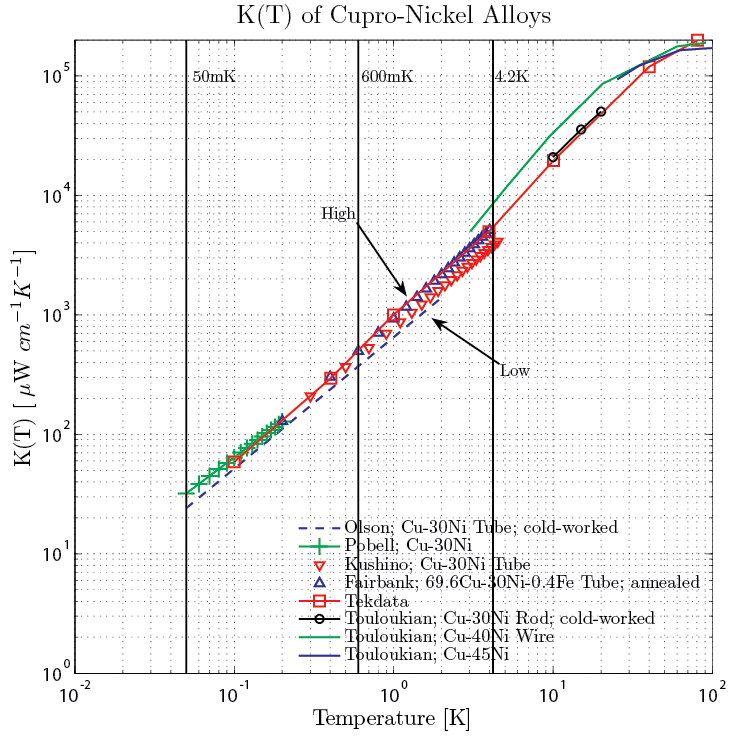
\includegraphics[width = 0.41\textwidth]{CuNi_graph.png}}
\caption{Thermal conductivity literature for trace material candidates. Variation between samples is largely due to varying thermo-mechanical treatment after production. In (b), Tekdata and Akerib measurements were performed on same wires used in CDMS Charge readout coaxes. In (d), Stainless alloys with similar composition to SS316 were used. Arrows indicate data sets used for graph in Section 1.2.}
\end{centering}
\end{figure}

\newpage
\section{Fluctuation in Resistance for Ti15-3-3-3 Trace}
The transition temperature of Ti 15-3-3-3 into its superconducting state is 3.89K \cite{wik}. If this material were used as a trace from the 4K stage to the Still of our towers, a portion of the trace would be in a normal state. This would give the line a resistance. Assuming the resistance of the line is low (tens of ohms), this is not a concern ; Fluctuating resistance, however, is a concern. As power loads to the fridge stages vary (from LED heating, circulation changes, etc.), the temperature gradient along the traces will vary as well. This will cause more/less of the line to be in a superconducting state -- varying resistance. The magnitude of these changes was calculated.

\begin{figure}[h]
\centering
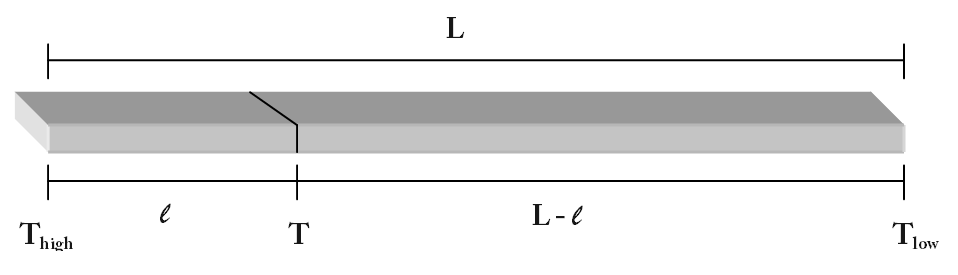
\includegraphics[width = .5\textwidth]{Ti15333_trace_resistivity_section.png}
\caption{}
\end{figure}

\subsection{Determining the Temperature Profile for Ti 15-3-3-3 Traces}
The temperature profile along a Ti 15-3-3-3 trace was calculated, assuming steady-state planar heat flow. To do this, consider the trace in two sections -- one with length $l$ and the other with length $L-l$, where $L$ is the overall length of the trace, as shown in Figure 10. In steady-state, the power through these two sections will be equal, so
\begin{eqnarray}
\frac{A}{l}\int_{T}^{T_{high}} k(T)dT = P = \frac{A}{L - l}\int_{T_{low}}^{T} k(T)dT
\end{eqnarray}
where A is the cross-sectional area of the trace, $T_{high}$ and $T_{low}$ are the temperatures of the 4K stage and Still respectively, $T$ is the temperature at a length $l$ along the trace, and $k(T)$ is the thermal conductivity of the trace. After rearranging this becomes,
\begin{eqnarray}
\frac{l}{L-l} = \frac{\int_{T_{low}}^{T} k(T)dT}{\int_{T}^{T_{high}} k(T)dT}
\end{eqnarray}
which can be integrated to find the temperature at any point $l$ along the trace. Since the Ti 15-3-3-3 thermal conductivity had to be numerically integrated, T values were picked in $T \in [T_{low},T_{high}]$ and the corresponding $l$ values were found. Figure 11 shows the temperature profile for a 9.24cm trace with $T_{high} = 4.2K$ and $T_{low}=0.6K$.

\begin{figure}[h]
\centering
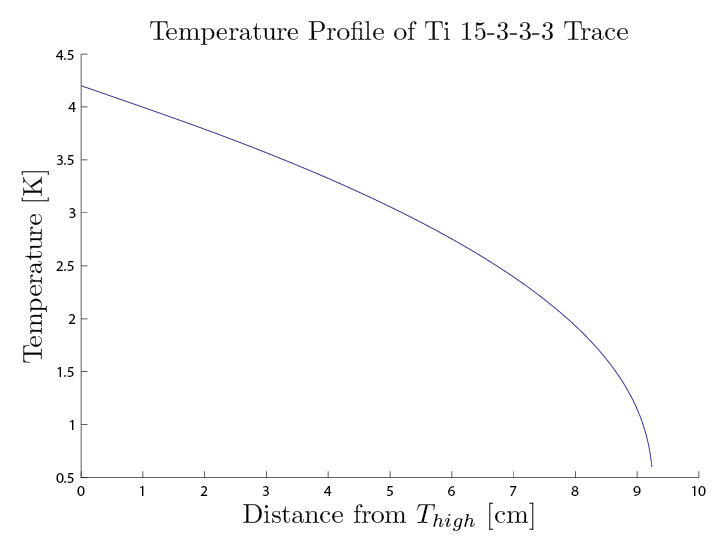
\includegraphics[width = .5\textwidth]{Ti153_T_Profile.png}
\caption{}
\end{figure}

\subsection{Resistivity of Ti 15-3-3-3}
The resistance of Ti 15-3-3-3 was measured by P. Wikus et al. Using the given dimensions, we converted to resistivity. This was then fitted to an equation to enable us to find the resistivity of Ti 15-3-3-3 as a function of temperature. The fitted resistivity is shown in Figure 12.

\begin{figure}[h]
\centering
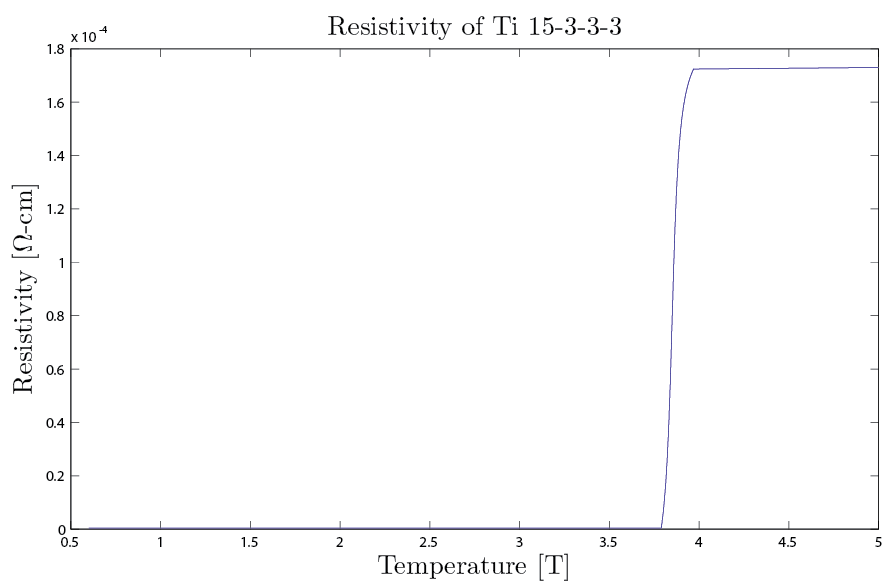
\includegraphics[width = .6\textwidth]{Ti_Resistivity.png}
\caption{Resistivity of Ti 15-3-3-3 showing $T_c$ at 3.89K}
\end{figure}

\subsection{Total Resistance of Trace}

Combining the resistivity and temperature profiles, the trace was subdivided into sections, each assigned a length, and the resistance was calculated for each. From this, the total resistance of the line was calculated. We find,

\begin{table}[h]
\begin{threeparttable}
\begin{tabular}{lcr}
\toprule
\multicolumn{2}{r}{Total Resistance [$\Omega$]} \\
\midrule
5K - 1K & $\rightarrow$ & 13.60 \\
4.2K - 0.6K & $\rightarrow$ & 5.64 \\
\bottomrule
\end{tabular}
\end{threeparttable}
\end{table}

\noindent With a total fluctuation of \bf{7.96 $\Omega$}.


\restoregeometry
\newpage
\bibliography{conductivity}

\end{document}

